\documentclass[10pt]{article}

\usepackage[margin=1in]{geometry} 
\usepackage{amsmath,amsthm,amssymb,bbm,subcaption,graphicx,float,physics,listings,fontspec,color}
\usepackage{tikz}

\usepackage{xeCJK}%据 @李清  改
\setCJKmainfont[BoldFont=SimHei, ItalicFont=KaiTi]{SimSun}
\setCJKmonofont{KaiTi}

\newfontfamily\Consolas{Consolas}
\definecolor{grey}{rgb}{0.9,0.9,0.9}
\lstset{basicstyle=\ttfamily, breaklines=true, numbers=left, numberstyle=\ttfamily, backgroundcolor=\color{grey}\ttfamily, keywordstyle=\color{blue}\ttfamily, stringstyle=\color{red}\ttfamily, commentstyle=\color{green}\ttfamily}
\DeclareMathOperator*{\argmin}{arg\,min}
\DeclareMathOperator*{\argmax}{arg\,max}
\DeclareMathOperator*{\Conv}{\mathop{\scalebox{1.5}{\raisebox{-0.2ex}{$\ast$}}}}
\DeclareMathOperator*{\vari}{var}

\begin{document}


% --------------------------------------------------------------
%                         Start here
% --------------------------------------------------------------
 
%\renewcommand{\qedsymbol}{\filledbox}
 
\title{\textbf{Report on Project 3}}%replace X with the appropriate number
\author{Zhunxuan Wang, 13300180086\\ %replace with your name
School of Mathematical Sciences} %if necessary, replace with your course title

\maketitle
\section{Recurrent Neural Network}
\subsection{Basic RNN Cell}
RNN is an efficient model to deal with sequential information. For each node in the same layer, \textit{recurrent} means they perform the same task for every element in the sequence, with the output being depended on the previous computations (memory) \cite{lecun2015deep}
\begin{figure}[H]
\centering
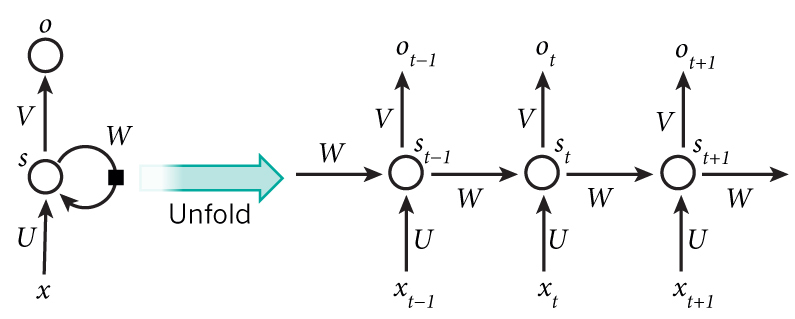
\includegraphics[scale=.5]{rnn.jpg}
\caption{The RNN and its Unfolding}
\label{rnn}
\end{figure}
The above diagram shows the unfolding of basic RNN, of which each node shares the same parameters. The formulas dominating the calculation are expressed as follows
\begin{itemize}
\item $\mathbf{x}_t$ is the input vector (i.e. word embedding) at time step $t$.
\item $\mathbf{s}_t$ is the hidden state (memory) at time step $t$, which is dominated by the previous hidden state and the input vector
$$\mathbf{s}_t = f\left(\mathbf{W}\mathbf{s}_{t-1} + \mathbf{U}\mathbf{x}_t\right)$$
where $f$ is generally a non-linear function (e.g. $\tanh$, \texttt{ReLu})
\item $\mathbf{o}_t$ is the output vector, which is dominated by the current hidden state
$$\mathbf{o}_t = g\left(\mathbf{V}\mathbf{s}_t\right)$$
where $g$ depends on what we need (e.g. \texttt{softmax} for obtaining the probability of each words).
\item $\mathbf{U}$, $\mathbf{V}$, $\mathbf{W}$ are the shared parameters, which are the parameters of a basic RNN cell.
\end{itemize}
\subsection{Basic LSTM Cell}
Long short-term memory (LSTM) \cite{hochreiter1997long} is a special kind of RNN, which is capable of remember long term dependencies. A basic LSTM cell is shown as follows
\begin{figure}[H]
\centering
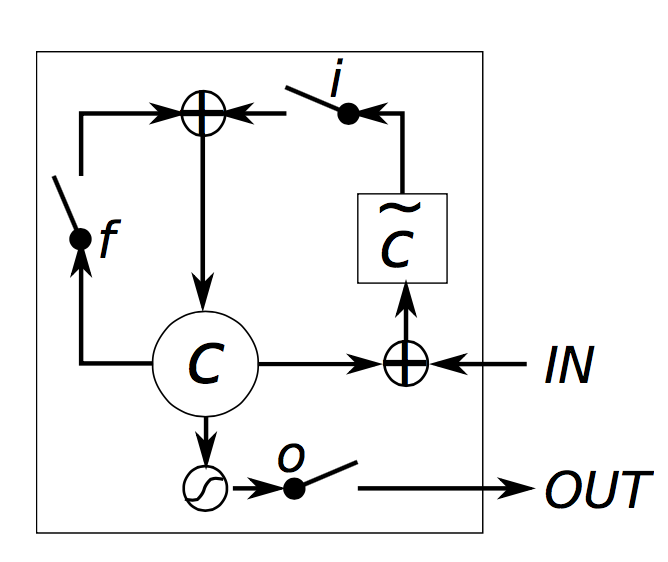
\includegraphics[scale=.6]{lstm.png}
\caption{Basic Structure of an LSTM Cell}
\label{lstm}
\end{figure}
As the diagram shows, we introduce $\mathbf{i}_t$, $\mathbf{f}_t$, $\mathbf{o}_t$, and $\mathbf{c}_t$, $\tilde{\mathbf{c}}_t$ of which the definition and the formula are expressed as follows
\begin{itemize}
\item $\mathbf{i}_t$, $\mathbf{f}_t$, $\mathbf{o}_t$ are the input, forget and output gates respectively. They have the same form but different parameters
\begin{align*}
& \mathbf{i}_t = \sigma\left(\mathbf{W}_{\text{i}}\mathbf{s}_{t-1} + \mathbf{U}_{\text{i}}\mathbf{x}_{t}\right) \\
& \mathbf{f}_t = \sigma\left(\mathbf{W}_{\text{f}}\mathbf{s}_{t-1} + \mathbf{U}_{\text{f}}\mathbf{x}_{t}\right) \\
& \mathbf{o}_t = \sigma\left(\mathbf{W}_{\text{o}}\mathbf{s}_{t-1} + \mathbf{U}_{\text{o}}\mathbf{x}_{t}\right)
\end{align*}
where $\mathbf{s}_t$, $\mathbf{x}_t$ are the hidden state and the input vector at time step $t$, $\mathbf{W}_{\text{i}, \text{f}, \text{o}}$ and $\mathbf{U}_{\text{i}, \text{f}, \text{o}}$ are the parameters of each gate.
\item $\tilde{\mathbf{c}}_t$ is the new candidate value, which could be added to the state
$$\tilde{\mathbf{c}}_t = \tanh\left(\mathbf{W}_{\text{c}}\mathbf{s}_{t-1} + \mathbf{U}_{\text{c}}\mathbf{x}_{t}\right)$$
of which the form is similar to the gates, but with a different activation function $\tanh$.
\item $\mathbf{c}_t$ is the internal memory, which is the sum of previous memory $\mathbf{c}_{t-1}$ multiplied by the forget gate $\mathbf{f}_t$, and the candidate value $\tilde{\mathbf{c}}_t$ multiplied by the input gate $\mathbf{i}_t$
$$\mathbf{c}_t = \mathbf{c}_{t-1} \circ \mathbf{f}_t + \tilde{\mathbf{c}}_t \circ \mathbf{i}_t$$
where $\circ$ is the operator of elementwise muliplication.
\item $\mathbf{s}_t$ is obtained by
$$\mathbf{s}_t = \tanh\left(\mathbf{c}_t\right) \circ \mathbf{o}_t\text{.}$$
\end{itemize}
Thereby the structure of a basic LSTM cell is established.
\subsection{Basic GRU Cell}
The structure behind a basic GRU (Gated Recurrent Unit) cell is quite similar to that of a basic LSTM cell
\begin{figure}[H]
\centering
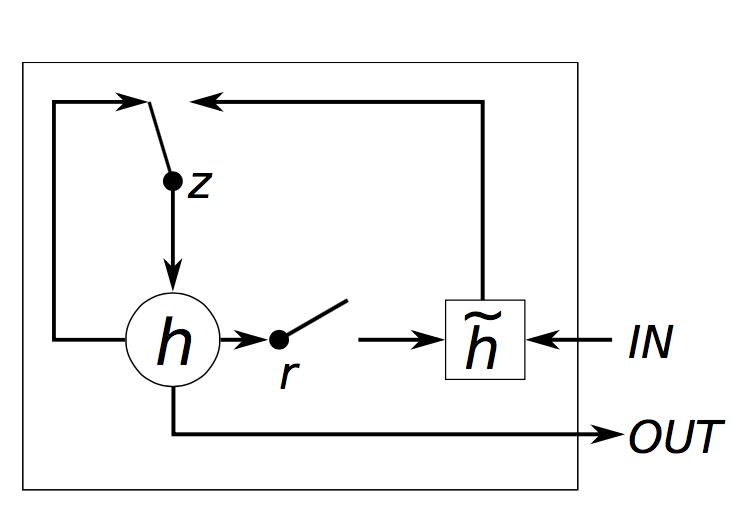
\includegraphics[scale=.6]{gru.png}
\caption{Basic Structure of a GRU Cell}
\label{gru}
\end{figure}
As the diagram shows, we introduce $\mathbf{z}_t$, $\mathbf{r}_t$, and $\mathbf{h}_t$, $\tilde{\mathbf{h}}_t$ of which the definition and the formula are expressed as follows \cite{chung2014empirical}
\begin{itemize}
\item $\mathbf{z}_t$, $\mathbf{r}_t$ are the update and reset gates respectively. They have the same form but different parameters
\begin{align*}
& \mathbf{z}_t = \sigma\left(\mathbf{W}_{\text{z}}\mathbf{s}_{t-1} + \mathbf{U}_{\text{z}}\mathbf{x}_{t}\right) \\
& \mathbf{r}_t = \sigma\left(\mathbf{W}_{\text{r}}\mathbf{s}_{t-1} + \mathbf{U}_{\text{r}}\mathbf{x}_{t}\right)
\end{align*}
where $\mathbf{s}_t$, $\mathbf{x}_t$ are the hidden state and the input vector at time step $t$, $\mathbf{W}_{\text{z}, \text{r}}$ and $\mathbf{U}_{\text{z}, \text{r}}$ are the parameters of each gate.
\item $\tilde{\mathbf{h}}_t$ is the new candidate activation
$$\tilde{\mathbf{h}}_t = \tanh\left(\mathbf{W}_{\text{h}}\left(\mathbf{s}_{t-1} \circ \mathbf{r}_t\right) + \mathbf{U}_{\text{h}}\mathbf{x}_{t}\right)\text{.}$$
where $\circ$ is the operator of elementwise muliplication.
\item $\mathbf{s}_t$ is obtained by
$$\mathbf{s}_t = \mathbf{s}_{t-1} \circ \mathbf{z}_t + \tilde{\mathbf{h}}_t \circ \left(\boldsymbol{1} - \mathbf{z}_t\right)\text{.}$$
\end{itemize}
Thereby the structure of a basic GRU cell is established.
\clearpage
\subsection{\texttt{Seq2seq} Generator}
To generate poems using RNN model, we chose to adopt \texttt{seq2seq} model \cite{sutskever2014sequence}, of which the main idea of this model is to feed the current input by the previous output. We adopted 2-layer RNN model to generate poems
\begin{figure}[H]
\centering
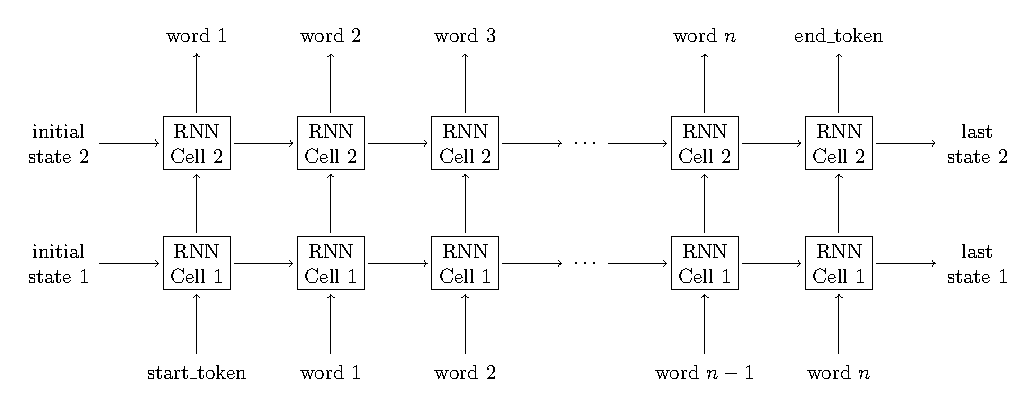
\includegraphics[scale=.8]{seq2seq.pdf}
\caption{An Example of Poems Generating}
\label{seq2seq}
\end{figure}
As we observe from the graph above, the generating began with feeding input by a start token. After that, the input of each iteration would be fed by the previous output, and the incoming state would be the previous state. When it came to the last word, the generating would end with an end token.\par
It is worth mentioning that, if we specify a word to begin, the input after the start token will be the specific word.
\section{Experimental Results}
Setting the loss function the cross entropy of prediction and one-hot target, choosing LSTM as the RNN cell, the 2-layer RNN model was trained after $50$ epochs, based on the dataset \texttt{poems.txt}.\par
we specified $8$ words to start with, and the poems generated are shown as follows
\begin{figure}[H]
\centering
\begin{subfigure}[t]{0.24\textwidth}
\centering
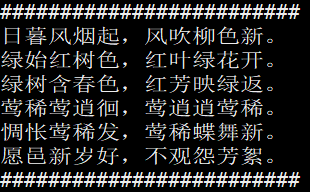
\includegraphics[scale=.65]{poems_1.png}
\caption{日}
\label{poems_1}
\end{subfigure}%
~
\begin{subfigure}[t]{0.23\textwidth}
\centering
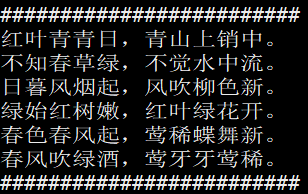
\includegraphics[scale=.65]{poems_2.png}
\caption{红}
\label{poems_2}
\end{subfigure}
~
\begin{subfigure}[t]{0.23\textwidth}
\centering
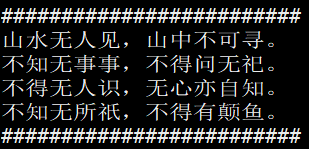
\includegraphics[scale=.65]{poems_3.png}
\caption{山}
\label{poems_3}
\end{subfigure}
~
\begin{subfigure}[t]{0.23\textwidth}
\centering
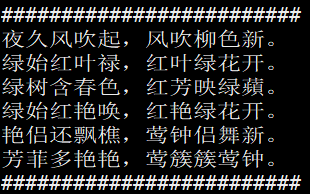
\includegraphics[scale=.65]{poems_4.png}
\caption{夜}
\label{poems_4}
\end{subfigure}
\vskip\baselineskip
\centering
\begin{subfigure}[t]{0.24\textwidth}
\centering
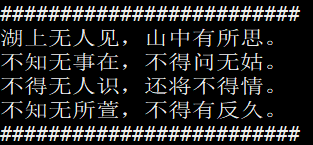
\includegraphics[scale=.65]{poems_5.png}
\caption{湖}
\label{poems_5}
\end{subfigure}%
~
\begin{subfigure}[t]{0.23\textwidth}
\centering
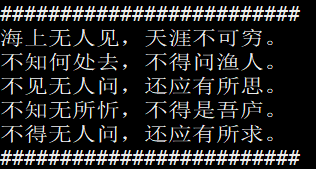
\includegraphics[scale=.65]{poems_6.png}
\caption{海}
\label{poems_6}
\end{subfigure}
~
\begin{subfigure}[t]{0.23\textwidth}
\centering
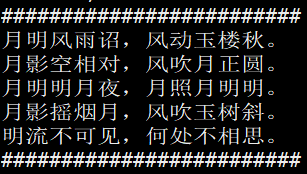
\includegraphics[scale=.65]{poems_7.png}
\caption{月}
\label{poems_7}
\end{subfigure}
~
\begin{subfigure}[t]{0.23\textwidth}
\centering
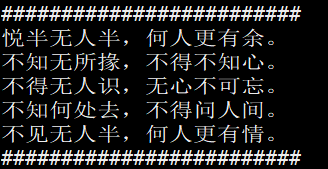
\includegraphics[scale=.65]{poems_8.png}
\caption{悦}
\label{poems_8}
\end{subfigure}
\caption{LSTM-Generated Poems Based on \texttt{poems.txt}}
\end{figure}
As we observe from the poems above, they are all five-character poems, and the statement of the generated poems is relatively fluent. However the logic in the context did not make much sense, and too many words repeated.\par
Retraining the model based on the previous model and the new \texttt{tangshi.txt} dataset, a new set of poems were generated, as the figures above show
\begin{figure}[H]
\centering
\begin{subfigure}[t]{0.24\textwidth}
\centering
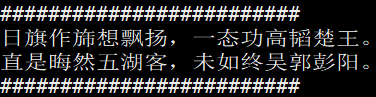
\includegraphics[scale=.6]{tangshi_1.png}
\caption{日}
\label{tangshi_1}
\end{subfigure}%
~
\begin{subfigure}[t]{0.23\textwidth}
\centering
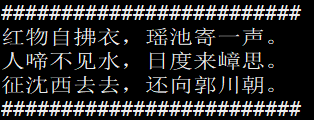
\includegraphics[scale=.6]{tangshi_2.png}
\caption{红}
\label{tangshi_2}
\end{subfigure}
~
\begin{subfigure}[t]{0.23\textwidth}
\centering
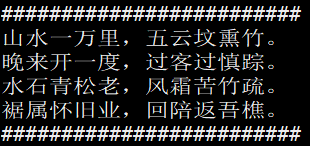
\includegraphics[scale=.6]{tangshi_3.png}
\caption{山}
\label{tangshi_3}
\end{subfigure}
~
\begin{subfigure}[t]{0.23\textwidth}
\centering
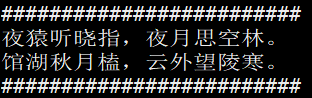
\includegraphics[scale=.6]{tangshi_4.png}
\caption{夜}
\label{tangshi_4}
\end{subfigure}
\vskip\baselineskip
\centering
\begin{subfigure}[t]{0.24\textwidth}
\centering
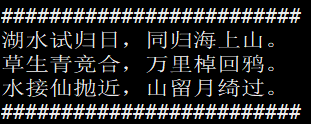
\includegraphics[scale=.6]{tangshi_5.png}
\caption{湖}
\label{tangshi_5}
\end{subfigure}%
~
\begin{subfigure}[t]{0.23\textwidth}
\centering
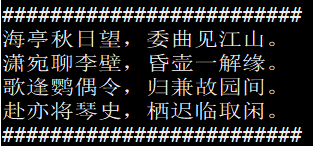
\includegraphics[scale=.6]{tangshi_6.png}
\caption{海}
\label{tangshi_6}
\end{subfigure}
~
\begin{subfigure}[t]{0.23\textwidth}
\centering
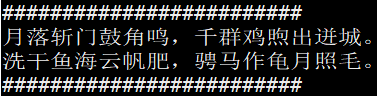
\includegraphics[scale=.6]{tangshi_7.png}
\caption{月}
\label{tangshi_7}
\end{subfigure}
~
\begin{subfigure}[t]{0.23\textwidth}
\centering

\includegraphics[scale=.6]{tangshi_8.png}
\caption{悦}
\label{tangshi_8}
\end{subfigure}
\caption{LSTM-Generated Poems Based on \texttt{poems.txt} and \texttt{tangshi.txt}}
\end{figure}
As we observe from the poems above, seven-character poems appeared, and the statement of the generated poems and the logic in the context is more fluent than before. Furthermore, the number of repeating words reduced a lot, and the efficiency on antithesis improved. In general, the model based on \texttt{poems.txt} and \texttt{tangshi.txt} is more efficient than that based on only \texttt{poems.txt}.
\section{Comparison between basicRNN, LSTM and GRU}
LSTM and GRU are gated mutants of RNN structure. They all perform well on poem generator model training, and better than basic RNN structure, with reference to the total train loss mean in the last epoch (when reaching the convergence state) $L$ (as the following table shows, only on \texttt{poems.txt})
\begin{center}
\begin{tabular}{|c|c|c|c|}
\hline
 & basicRNN & LSTM & GRU\\
\hline
$L$ & $5.819501$ & $4.082350$ & $4.222888$ \\
\hline
\end{tabular}
\end{center}
From the table we can infer that the performance by LSTM and GRU are close (LSTM are a little better than GRU), each of which performs better than basic RNN (on \texttt{poems.txt}).\par
The poems generated by basic RNN and GRU are in the appendix \ref{app_A}. As we can obtain from the poems, the poems generated by basic RNN are very short and monotonous, and the poems generated by GRU make more sense that by basic RNN, but they lack more logic in context and have more repeating words than LSTM-generated poems.
%\begin{figure}[H]
%\centering
%\begin{minipage}[b]{0.45\textwidth}
%\centering
%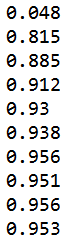
\includegraphics[scale=1.]{fig1.png}
%\label{fig3}
%\end{minipage}
%\
%\begin{minipage}[b]{0.45\textwidth}
%\centering
%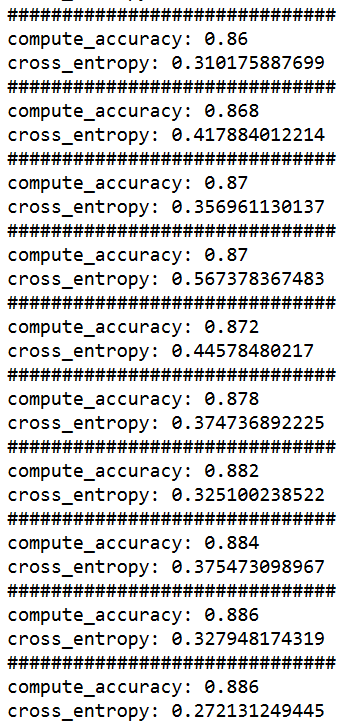
\includegraphics[scale=1.]{fig2.png}
%\label{fig4}
%\end{minipage}
%\caption{The Screenshots of Running Result}
%\end{figure}
\clearpage
\bibliographystyle{plain}
\bibliography{ref}
\clearpage
\appendix
\section{Poems by basicRNN and GRU}
\begin{figure}[H]
\centering
\begin{subfigure}[t]{0.24\textwidth}
\centering
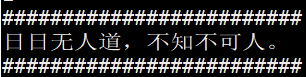
\includegraphics[scale=.6]{rnn_1.png}
\caption{日}
\label{rnn_1}
\end{subfigure}%
~
\begin{subfigure}[t]{0.23\textwidth}
\centering
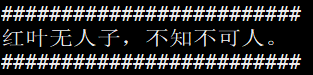
\includegraphics[scale=.6]{rnn_2.png}
\caption{红}
\label{rnn_2}
\end{subfigure}
~
\begin{subfigure}[t]{0.23\textwidth}
\centering
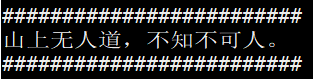
\includegraphics[scale=.6]{rnn_3.png}
\caption{山}
\label{rnn_3}
\end{subfigure}
~
\begin{subfigure}[t]{0.23\textwidth}
\centering
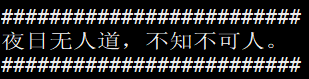
\includegraphics[scale=.6]{rnn_4.png}
\caption{夜}
\label{rnn_4}
\end{subfigure}
\vskip\baselineskip
\centering
\begin{subfigure}[t]{0.24\textwidth}
\centering
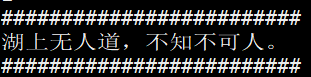
\includegraphics[scale=.6]{rnn_5.png}
\caption{湖}
\label{rnn_5}
\end{subfigure}%
~
\begin{subfigure}[t]{0.23\textwidth}
\centering
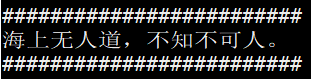
\includegraphics[scale=.6]{rnn_6.png}
\caption{海}
\label{rnn_6}
\end{subfigure}
~
\begin{subfigure}[t]{0.23\textwidth}
\centering
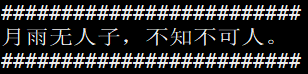
\includegraphics[scale=.6]{rnn_7.png}
\caption{月}
\label{rnn_7}
\end{subfigure}
~
\begin{subfigure}[t]{0.23\textwidth}
\centering
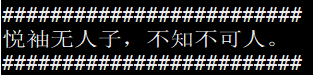
\includegraphics[scale=.6]{rnn_8.png}
\caption{悦}
\label{rnn_8}
\end{subfigure}
\caption{basicRNN-Generated Poems Based on \texttt{poems.txt}}
\end{figure}
\begin{figure}[H]
\centering
\begin{subfigure}[t]{0.24\textwidth}
\centering
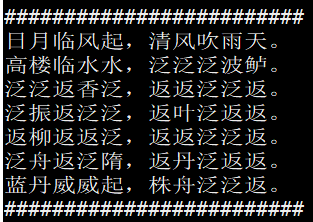
\includegraphics[scale=.6]{gru_1.png}
\caption{日}
\label{gru_1}
\end{subfigure}%
~
\begin{subfigure}[t]{0.23\textwidth}
\centering
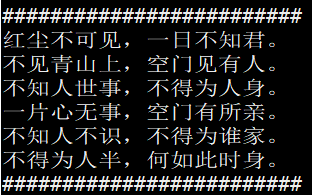
\includegraphics[scale=.6]{gru_2.png}
\caption{红}
\label{gru_2}
\end{subfigure}
~
\begin{subfigure}[t]{0.23\textwidth}
\centering
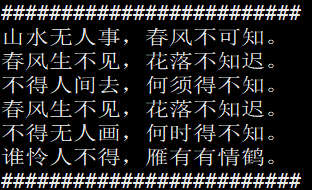
\includegraphics[scale=.6]{gru_3.png}
\caption{山}
\label{gru_3}
\end{subfigure}
~
\begin{subfigure}[t]{0.23\textwidth}
\centering
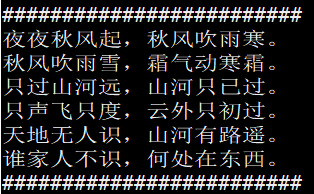
\includegraphics[scale=.6]{gru_4.png}
\caption{夜}
\label{gru_4}
\end{subfigure}
\vskip\baselineskip
\centering
\begin{subfigure}[t]{0.24\textwidth}
\centering
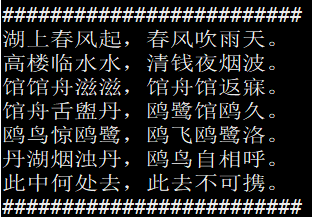
\includegraphics[scale=.6]{gru_5.png}
\caption{湖}
\label{gru_5}
\end{subfigure}%
~
\begin{subfigure}[t]{0.23\textwidth}
\centering
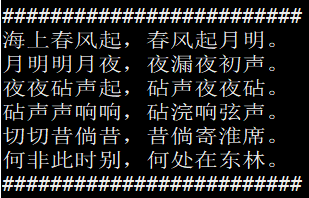
\includegraphics[scale=.6]{gru_6.png}
\caption{海}
\label{gru_6}
\end{subfigure}
~
\begin{subfigure}[t]{0.23\textwidth}
\centering
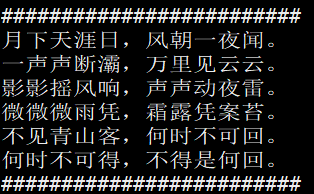
\includegraphics[scale=.6]{gru_7.png}
\caption{月}
\label{gru_7}
\end{subfigure}
~
\begin{subfigure}[t]{0.23\textwidth}
\centering
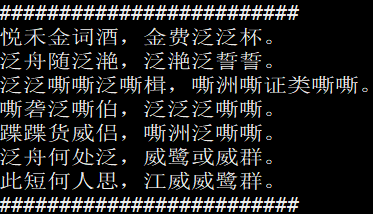
\includegraphics[scale=.6]{gru_8.png}
\caption{悦}
\label{gru_8}
\end{subfigure}
\caption{GRU-Generated Poems Based on \texttt{poems.txt}}
\end{figure}
\label{app_A}
\end{document}